%J�rn
\section{Fachkonzept}
Im \ref{ooa} wurde bereits das Klassendiagramm der Analysephase n�her erl�utert.
Bei der Implementierung auf Basis dieses Klassenmodells haben wir aber noch
einige �nderungen und Einschr�nkungen vorgenommen. Im volgenden Abschnitt werden
diese Unterschiede und dessen Hintergr�nde n�her erl�utert.

\subsection{Client-Server}
Die Client-Server Architektur, die bei unserem Planspiel angewandt wird,
erm�glicht es mehreren Spielern ihren Spielzug gleichzeitig zu absolvieren.
Zwar verringert dies die Wartezeitden der Spieler im Gegensatz zum
Hotseat-Modell, allerdings muss bei einem gemeinsamen Server und mehreren
Clienten darauf geachtet werden, dass es zu keinen Dateninkonsistenzen kommt.
An der ``Thread-per-Connection''-Methode hat sich seit der Analysephase (siehe
\ref{ooa}) nichts ge�ndert, weswegen hier darauf nicht n�her eingegangen wird.

In \ref{OOD-Map} ist die Klassenstruktur abgebildet, die alle Daten enth�lt, die
f�r alle Spieler interessant sind und indirekt auch von diesen ge�ndert werden
k�nnen. Um Dateninkonsistenz zu vermeiden werden alle �nderungen die ein Spieler
eingibt an den Server gesendet, dieser wertet die �nderungen aus �bertr�gt sie
gegebenenfalls in den entsprechenden Objekten. Zu Rundenbeginn wird nun die
gesamt Objektstruktur, die in einem Objekt der 'Map'-Klasse auf Serverseite
gespeichert ist, an alle Clients �bertragen. Dadurch, dass nur der Server solche
�nderungen vornehmen kann und diese auch nicht von verschiedenen
'Connection'-Threads gleichzeitig vorgenommen k�nnen (``Synchronized''), wird
die richtige Datenhaltung sichergestellt.

\begin{figure}
\centering
\centering
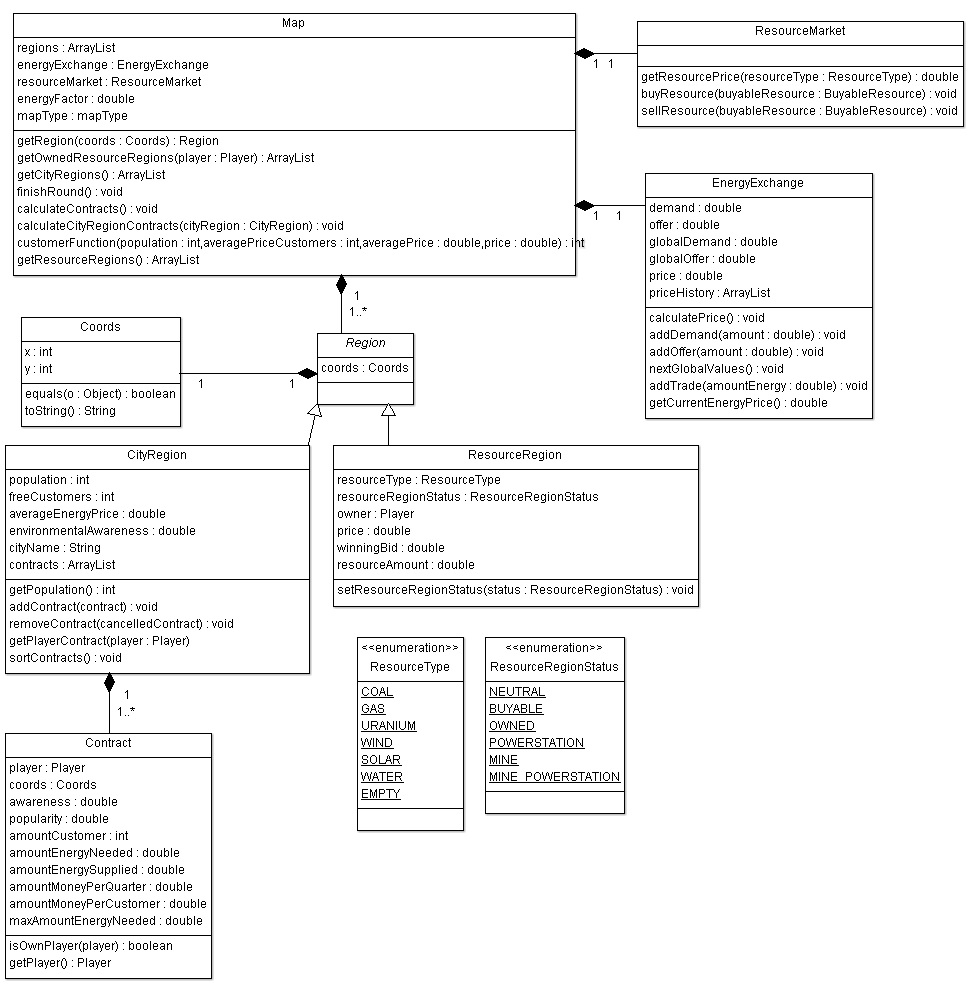
\includegraphics[width=1.1\textwidth]{se-wa-jpg/OOD-Map}
\caption{Klassendiagramm Kommunikationsklassen}
\label{OOD-Map}
\end{figure}

W�hrend der Analysephase war es angedacht, Vertr�ge mit einer Stadt unabh�ngig
vom Rundenende zu schlie�en. Diese Idee wurde w�hrend der Entwcklung verworfen,
so dass nun jeder Spieler seine Vertragsvorschl�ge dem Server w�hrend der Runde
zusendet, der Server nach der Runde die Kunden jedes Spielers
errechnet und zum n�chsten Rundenanfang diese den Spielern mitteilt.\\
Wie in \ref{OOD-Map} zu sehen ist, haben wir uns deswegen dazu entschieden den
'Contract', der vorher unter dem Unternehmen in dem Bereich der Beziehungen zu
den Regionen angeordnet war, nun der 'Map' und darin der 'CityRegion' zu
unterordnen.\\
Diese �nderung in der Struktur der Fachlogik erlaubt es dem Server weiterhin,
alle Daten, die jede Runde den Spielern zugeschickt werden, in einer einzigen
Objektstruktur zu �bertragen.
Dies erm�glicht zum einen eine einfache Kommunikation vom Server zum Client und
zum anderen kann nun auch der Client alle wichtigen �nderungen der Runde aus
einem einzigen Objekt auslesen, in dem er die neu erhaltene 'Map' mit der
vorhandenen aus der vergangenen Runde vergleicht.
